\documentclass[Bachelorarbeit.tex]{subfiles}
\begin{document}

\graphicspath{{./figures/hypothesis/}}	%specifying the folder for the figures

\chapter{Hypothesis}
\label{ch:hypothesis}

In this chapter the question of the importance of fully-connectedness for reaching the equilibrium is raised where the question is whether it is really necessary to have a fully-connected network to reach equilibrium or not. We challenge this and claim that a much lower connectivity but a very special one is required and present a definition for it in a hypothesis which states that if a network satisfies the postulated properties of the hypothesis then using this network in the simulation will result in approaching the same equilibrium as found in fully-connected networks.

\section{Definition}

\begin{equation}
\begin{split}
\textit{fully-connectedness equilibrium} \iff \\
\forall \: \textit{agent-pairs} \: (a_{1},a_{n}) \: \exists \:  \textit{path} \: P \: \{a_{1}, a_{2}, ... , a_{n-1}, a_{n}\} \: | \: h(a_{i}) < h(a_{i+1})
\end{split}
\end{equation}

\newtheorem{conj}{Conjecture}

\begin{conj}
If and only if for all agents exists a path between two agents in which each visited agent has a larger optimism factor than the previous one then the same equilibrium as in fully-connectedness will be reached.
\end{conj}

The most minimal configuration of agents which satisfies this hypothesis is a graph of agents where each agent is connected to the agent with the next higher optimism-factor. This is the same as the Ascending-Connected topology - see appendix \ref{app:topologies} - which is the major network of interest in this thesis (besides the fully-connected one) as it is the most minimal topology which satisfies the hypothesis.

\section{Motivation}
The motivation behind the hypothesis is the fact that according to the double-auction definition - see chapter \ref{ch:theory} - for a match to happen the buyer-price must be larger or equal to the seller-price. This can only be the case when the buyer has a higher optimism-factor than the seller due the way agents place their prices - see chapter \ref{ch:leverageCycle}.

\subsection{Proof}
The proofs are given for the Asset/Cash market only because the equations of the Loan/Cash market work exactly the same way where only the absolute numbers are different. The Asset/Bond market is the same too as the limit-price is just the ratio of the limit-prices of asset and bond thus resulting in the same linear ordering of the limit-prices. TODO: stimmt nicht

\paragraph{Illustrating the matching ranges}
In figure \ref{fig:MATCHING_BUYER_SELLER_RANGES} the price-ranges of both a seller and buyer are given where h(s) and h(b) denote the optimism-factors of the seller and buyer respectively. The seller places its offerings in the price-range of [h(s)..pU] as it wants to sell the good above the expected price to make a profit. The buyer places its offerings in the price-range of [pD..h(b)] as it wants to buy the goods below the expected price to make a profit. The resulting matching-range on which the prices can meet - again buyer-price $\geq$ seller-price - is marked by the red rectangle. It is easy to see that a match with these mechanics can occur only if the optimism-factor of the buyer h(b) is strictly higher than the one of the seller h(s).

\begin{figure}[H]
	\centering
  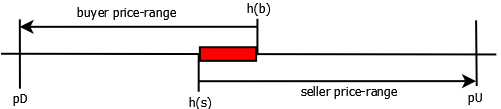
\includegraphics[width=1.0\textwidth, angle=0]{MATCHING_BUYER_SELLER_RANGES.png}
  	\caption{Matching of buyers and sellers price-ranges. The red rectangle marks the matching-range.}
	\label{fig:MATCHING_BUYER_SELLER_RANGES}
\end{figure}


\paragraph{Formal proof}
Proofing optimism of buyer is greater or equal than the optimism of the seller $h_B \geq h_S$ by showing the limit-price of the buyer is greater of equal the limit-price of the seller $limit_B \geq limit_S$.

either through proof by contradiction: assume a seller with a larger optimism than the buyer and show that the assumption that the utility-function must increase fails.

or through difference between the two utility functions of a buyer and a seller: difference is always larger or smaller (dependeing on the direction of subtraction) than zero.

TODO: hypothese beweisen
1. zeigen dass hypothese auf minimale vernetzung reduziert werden kann bzw. dass diese minimale vernetzung ausreicht. (über den vorhergehenden formal proof und dass limit-prices monoton steigen)
2. zeigen, dass lücken bei minimalster vernetzung an beliebiger stelkle zu widerspruch führt: gleichgewicht wird nicht erreicht. 

\subsubsection{Asset/Cash}
$limit_B = h_B + \frac{1}{5} - \frac{h_B}{5}$ \\
$limit_S = h_S + \frac{1}{5} - \frac{h_S}{5}$

\begin{proof}
\begin{align*}
	limit_S - limit_B \leq 0
	\\ (h_S + \frac{1}{5} - \frac{h_S}{5}) - ( h_B + \frac{1}{5} - \frac{h_B}{5} ) \leq 0
	\\ h_S + \frac{1}{5} - \frac{h_S}{5} - h_B - \frac{1}{5} + \frac{h_B}{5} \leq 0
	\\ 5h_S + 1 - h_S - 5h_B - 1 + h_B \leq 0
	\\ 4h_S - 4h_B \leq 0
	\\ h_S - h_B \leq 0		\tag*{can only hold if $h_B \geq h_S$}
\end{align*}
\end{proof}

\pagebreak
\subsubsection{Bond/Cash}
$limit_B = h_B \, V + \frac{1}{5} - \frac{h_B}{5}$ \\
$limit_S = h_S \, V + \frac{1}{5} - \frac{h_S}{5}$

\begin{proof}
\begin{align*}
	limit_S - limit_B \leq 0
	\\ (h_S \, V  + \frac{1}{5} - \frac{h_S}{5}) - ( h_B \, V  + \frac{1}{5} - \frac{h_B}{5} ) \leq 0
	\\ h_S \, V  + \frac{1}{5} - \frac{h_S}{5} -  h_B \, V  - \frac{1}{5} + \frac{h_B}{5} \leq 0
	\\ 5 h_S \, V  + 1 - h_S - 5h_B \, V  - 1 + h_B \leq 0
	\\ 5 h_S \, V - 5h_B \, V - h_S + h_B \leq 0
	\\ 5V(h_S - h_B) - (h_S - h_B) \leq 0	\tag*{substituting $u = (h_S - h_B)$}
	\\ 5Vu - u \leq 0	\tag*{assuming $h_S > h_B$}	
	\\ \Rightarrow u > 0 \Rightarrow 5Vu - u > 0 		\tag*{violates the original assumption}	
	\\ \textit{proof by contradiction} \Rightarrow h_B \geq h_S
\end{align*}
\end{proof}

\pagebreak
\subsubsection{Asset/Bond}
$limit_B = \frac{h_B + \frac{1}{5} - \frac{h_B}{5}}{h_B \, V + \frac{1}{5} - \frac{h_B}{5}}$ \\
$limit_S = \frac{h_S + \frac{1}{5} - \frac{h_S}{5}}{h_S \, V + \frac{1}{5} - \frac{h_S}{5}}$ \\

\begin{proof}
\begin{align*}
	limit_S - limit_B \leq 0
	\\ \frac{h_S + \frac{1}{5} - \frac{h_S}{5}}{h_S \, V + \frac{1}{5} - \frac{h_S}{5}} - \frac{h_B + \frac{1}{5} - \frac{h_B}{5}}{h_B \, V + \frac{1}{5} - \frac{h_B}{5}} \leq 0
	\\ (h_S + \frac{1}{5} - \frac{h_S}{5})(h_B \, V + \frac{1}{5} - \frac{h_B}{5}) - (h_B + \frac{1}{5} - \frac{h_B}{5})(h_S \, V + \frac{1}{5} - \frac{h_S}{5}) \leq 0													
	\\ substituting \; S = \frac{1}{5} - \frac{h_S}{5}, B = \frac{1}{5} - \frac{h_B}{5}
	\\ (h_S + S)(h_B \, V + B) - (h_B + B)(h_S \, V + S) \leq 0
	\\ h_S \, h_B \, V + h_S \, B + S \, h_B \, V + BS - (h_B \, h_S \, V + h_B \, S + B \, h_S \, V + BS) \leq 0
	\\ h_S \, h_B \, V + h_S \, B + S \, h_B \, V + BS - h_B \, h_S \, V - h_B \, S - B \, h_S \, V - BS \leq 0
	\\ h_S \, B + S \, h_B \, V - h_B \, S - B \, h_S \, V \leq 0
	\\ h_S \, B - h_B \, S + V(h_B \, S - h_S \, B ) \leq 0 
	\\ h_S(\frac{1}{5} - \frac{h_B}{5}) - h_B(\frac{1}{5} - \frac{h_S}{5}) + V(h_B(\frac{1}{5} - \frac{h_S}{5}) - h_S(\frac{1}{5} - \frac{h_B}{5})) \leq 0
	\\ \frac{h_S}{5} - \frac{h_S \, h_B}{5} - \frac{h_B}{5} + \frac{h_B \, h_S}{5} + \frac{h_B \, V}{5} - \frac{h_B \, h_S \, V}{5} - \frac{h_S \, V}{5} + \frac{h_S \, h_B \, V}{5} \leq 0 
	\\ \frac{h_S}{5} - \frac{h_B}{5} + \frac{h_B \, V}{5} - \frac{h_S \, V}{5} \leq 0
	\\ h_S - h_B + h_B \, V - h_S \, V \leq 0 
	\\ h_S( 1 - V ) + h_B( -1 + V ) \leq 0 
	\\ substituting \; x = h_S( 1 - V ), y = h_B( -1 + V )
	\\ x + y \leq 0 									
	\\ \textit{assume V linear in range of} \; [0..1]
	\\ x = [h_S..0] \Rightarrow x \geq 0 
	\\ y = [-h_B..0] \Rightarrow y \leq 0
	\\ \Rightarrow x + y \leq 0 \iff h_B \geq h_S
\end{align*}
\end{proof}

\subsection{Proof of monotony of limit-functions}
\subsubsection{Asset/Cash market}
\begin{proof}
\begin{align*}
	limit_{asset} = h \, pU + (1-h) pD		\tag*{pU = 1, pD = 0.2}
	\\ = h + (1 - h)0.2
	\\ = h + \frac{1}{5} - \frac{h}{5}		\tag*{$\frac{\mathrm d}{\mathrm d h}$}
	\\ = 1 - \frac{1}{5}
		&= \frac{4}{5}
\end{align*}

constant, positive slope implies a monotony increasing limit-function over the range of the real numbers. QED
\end{proof}

\subsubsection{Bond/Cash market}
\begin{proof}
\begin{align*}
	limit_{bond} = h \, V + (1-h) pD			\tag*{pD = 0.2}
	\\ = h \, V + (1 - h)0.2
	\\ = h \, V + \frac{1}{5} - \frac{h}{5}		\tag*{$\frac{\mathrm d}{\mathrm d h}$}
	\\ = V - \frac{1}{5}
\end{align*}

V is constant => constant, positive slope implies a monotony increasing limit-function were $V >= \frac{1}{5}$. QED
\end{proof}

\subsubsection{Asset/Bond market}
\begin{proof}
\begin{align*}
	limit_{asset/bond} = \frac{h \, pU + (1-h) pD}{h \, V + (1-h) pD} 				\tag*{pU = 1, pD = 0.2}
	\\ = \frac{h + \frac{1}{5} - \frac{h}{5}}{h \, V + \frac{1}{5} - \frac{h}{5}}	\tag*{$\frac{\mathrm d}{\mathrm d h}$}
	\\ = - \frac{5(V-1)}{(h(5V-1)+1)^2}									\tag*{assume h and V in range [0..1]}
	\\ \Rightarrow 5(V-1) \leq 0
	\\ \Rightarrow (h(5V-1)+1)^2 \geq 0
	\\ \Rightarrow - \frac{5(V-1}{(h(5V-1)+1)^2} \geq 0 			\tag*{for h and V in range [0..1]}
\end{align*}

positive slope implies a monotony increasing limit-function. QED

\end{proof}

\section{Predictions}
The following topologies found in appendix \ref{app:topologies} satisfy the definition of the hypothesis:
 
\begin{itemize}
\item Fully-Connected
\item Half-Fully connected
\item Ascending-Connected
\item Ascending-Connected with all kind of short-cuts
\item Erdos-Renyi and Watts-Strogatz with the correct parametrization by pure chance.
\end{itemize}

It is expected that according to the hypothesis all of these topologies will reach the equilibrium found in fully-connectedness. All other topologies do not satisfy the hypothesis and are expected to clearly fail reaching the equilibrium of the Fully-Connected topology.

\medskip

See chapter \ref{ch:results} and \ref{ch:interpretation} whether the results reflect the hypothesis or not. 

\end{document}